\section{Training der Modelle}
Typischerweise haben weder Entscheidungsbaum basierte Klassifizierer noch FFNN Rückwärtskanten.
Neuronale Netze mit Rückwärtskanten werden als \textit{rekurrente Netze} (RNN) bezeichnet.
Abbildung \ref{fig:model_idea} zeigt, dass die Rückwärtskante genutzt wird, um das Klassifizierungsergebnis,
also den letzten Standort, bei der Feature-Extrahierung zu nutzen.
\newline
\newline
\begin{figure}[h!]
    \centering
    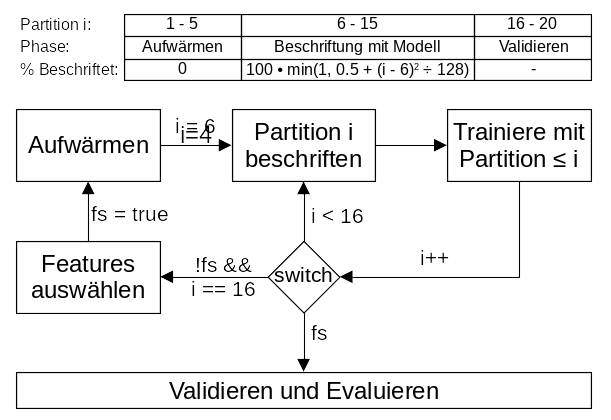
\includegraphics[width=\linewidth]{images/training_explained.png}
    \caption{Der Trainingsablauf des verfolgten Ansatzes.}
    \label{fig:training_explained}
\end{figure}
\newline
\begin{itemize}
    \item Zusammenhang zur Feedback Edge deutlich machen => Bessere Einleitung finden
    \item Trainieren in Phasen => Erklären wie es genau funktioniert?
    \item Warum trainieren wir in Phasen? => Erkläre, dass wir Klassifizierungsfehler lernen wollen, damit wir wieder zurückfinden.
    \item Sag das wir die Zyklen der einzelnen Pfade nutzen
    \item Werden mehr Trainingsdaten benötigt mit steigender Ort Anzahl? Wenn ja wie viel?
    \item Doppeltes Trainieren nach Analyse der Feature Importance.
    \item Warum machen wir das so?
    \item Zufälliges Relabeling im Training? Warum und wie funktionierts?
    \item Anteil der Daten der gerelabelt wird steigt mit Anzahl der Zyklen
\end{itemize}